\usetikzlibrary{calc}

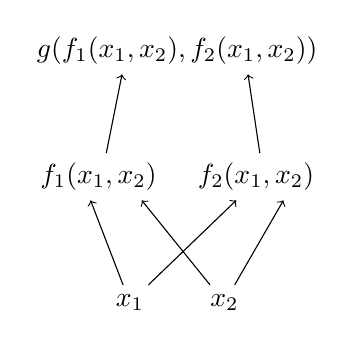
\begin{tikzpicture}
	\def\k{1.6}
	\node (g) at (0,1*\k) {$g(f_1(x_1,x_2),f_2(x_1,x_2))$};
 	\node (f1) at (-1,0*\k) {$f_1(x_1,x_2)$};
 	\node (f2) at (1,0*\k) {$f_2(x_1,x_2)$};
 	\node (x1) at (-0.6,-1*\k) {$x_1$};
 	\node (x2) at (0.6,-1*\k) {$x_2$};
 	
 	\path[<-] ($(g.south)+(-0.7,0)$) edge node {} ($(f1.north)+(.1,0)$);
 	\path[<-] ($(g.south)+(0.9,0)$) edge node {} ($(f2.north)+(.05,0)$);
 	\path[<-] ($(f1.south)+(-.1,0)$) edge node {} (x1);
 	\path[<-] ($(f1.south)+(.55,0)$) edge node {} (x2);
 	\path[<-] ($(f2.south)+(-.25,0)$) edge node {} (x1);
 	\path[<-] ($(f2.south)+(.35,0)$) edge node {} (x2);
 	
 	\def\labeltext{
 		Note:\\
 		$\;\;\;y_1=f_1(x_1,x_2)$\\
 		$\;\;\;y_2=f_2(x_1,x_2)$
 	}
% 	\node[draw,align=left,font=\large] at (4.3,0) {\labeltext};
\end{tikzpicture}
